
\section{Auswertung}

\subsection{Messung der Zeitkonstanten mit der Entladekurve}
Für die Bestimmung der Zeitkonstante des RC-Gliedes wird die Entladungskurve des Kondensators
mit Hilfe eines Oszillographen bestimmt.
Dem Thermodruck können die Messwerte für die Spannung
$U_c$ und die Temperatur $t$ entnommen werden.
Durch die lineare Regression kann die Steigung des Graphen ermittelt werden, wobei der Betrag
des Kehrwerts der Zeitkonstanten entspricht.

\begin{align}
m    &= -\frac{1}{RC}
\end{align}

Mithilfe der linearen Regression ergibt sich für die Zeitkonstatne RC
folgender Wert:
$RC = ( 0.000775\pm 0.000070) \, \su{s}$

\begin{table}
  \centering
  \caption{Entnommene Wertepaare für die Spannungsamplituden zu verschiedenen
          Zeitpunkten des Entladevorgangs}
  \label{tab:MessungA}
  \begin{tabular}{c c c}
    \toprule $t \,\, in \,\, \su{ms}$ & $U\ua{C} \,\, in \,\, \su{V}$ & $ln(U)$ \\
    \midrule
    0.0 & 3.6  & 1.28 \\
    0.2 & 2.48 & 0.91 \\
    0.4 & 2.16 & 0.77  \\
    0.6 & 1.68 & 0.52 \\
    0.8 & 1.28 & 0.25 \\
    1.0 & 0.96 & -0.04 \\
    1.2 & 0.8  &-0.22 \\
    1.4 & 0.56 & -0.58 \\
    1.6 & 0.48 & -0.73 \\
    1.8 & 0.32 & -1.14 \\
    2.0 & 0.24 & -1.43 \\
    2.2 & 0.24 & -1.43 \\
    2.4 & 0.16 & -1.83 \\
    2.6 & 0.08 & -2.53 \\
    2.8 & 0.08 & -2.53 \\
    3.0 & 0.08 & -2.53 \\
    3.2 & 0.08 & -2.53 \\
    3.4 & 0 & n. def. \\
    3.6 & 0 & n. def. \\
    3.8 & 0 & n. def. \\
    4.0 & 0 & n. def. \\
    4.2 & 0 & n. def. \\
    4.4 & 0 & n. def. \\
    4.6 & 0 & n. def. \\
    4.8 & 0 & n. def. \\

    \bottomrule
  \end{tabular}
\end{table}
\begin{figure}
  \centering
  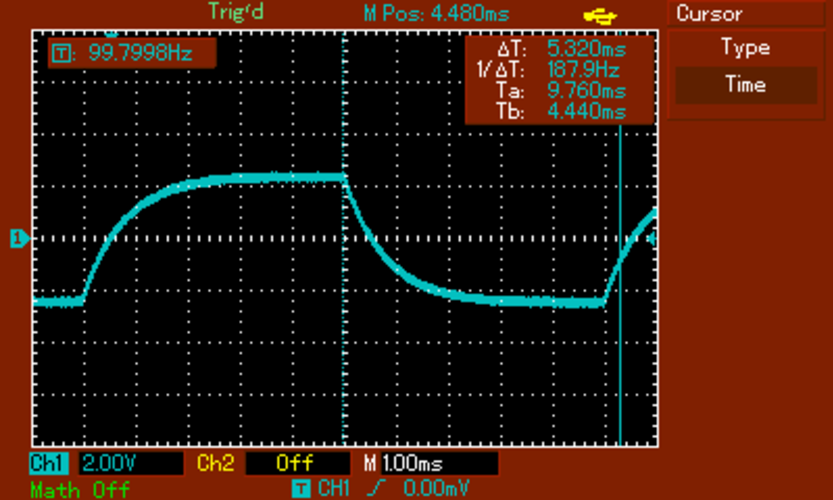
\includegraphics[width = 12 cm]{spannungentladen.pdf}
  \caption{Thermodruck der in Messung \ref{tab:MessungA} betrachteten Entladekurve}
  \label{fig:thermodruck}
\end{figure}

\begin{figure}
  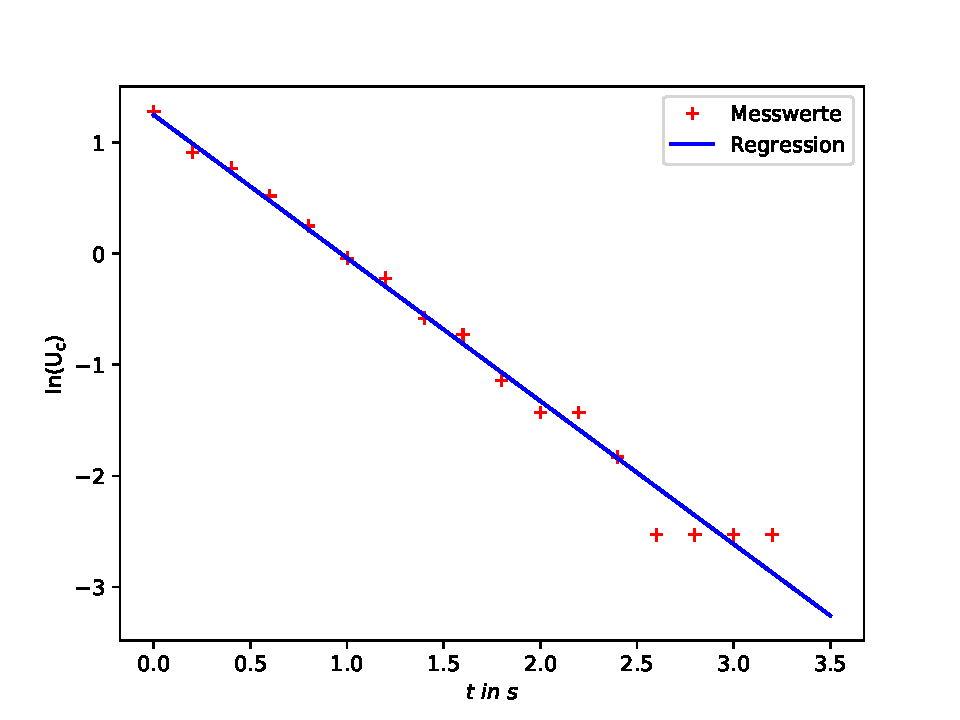
\includegraphics[width = 12 cm]{entladen.pdf}
  \caption{gemessene Werte für $U\ua{C}$ aufgetragen gegen die Zeit $t$}
  \label{fig:Messunga}
\end{figure}

\newpage
\subsection{Messung der Zeitkonstante über die Amplitude}

Für die Bestimmung der Zeitkonstante über die Amplitude werden dreißig Frequenzen
 untersucht.
Mit dem gemessen Wert für $U\ua{o}$ = $0.52V$ lässt sich der Quotient von
Amplitude und Eingangsspannung
bestimmen.

\begin{equation}
  \frac{A(\omega)}{U\ua{0}} = \frac{1}{ \sqrt{ 1 + \omega ^2 \cdot (RC)^2}}
  \label{eqn:FitMessungB}
\end{equation}
Aus Abbildung \ref{fig:Messungb} ergibt sich mithilfe der Regressionskurve
für die Zeitkonstante
der Wert:
\begin{equation*}
  RC = (0.000768 \pm 0.000013) \, \su{s} .
\end{equation*}
\begin{table}
  \centering
  \caption{Gemessene Spannungsamplituden der Kondensatorspannung für verschiedene
           angelegte Frequenzen $\omega$}
  \label{tab:MessungB}
  \begin{tabular}{ c c c }
    \toprule $\omega \,\, in \,\, \su{Hz}$ & A($\omega$) & A($\omega$)/U \\
    \midrule
    10 & 0.488 & 0.938 \\
    20 & 0.504 & 0.969 \\
    30 & 0.504 & 0.969 \\
    40 & 0.504 & 0.969 \\
    50 & 0.504 & 0.969 \\
    60 & 0.488 & 0.938 \\
    70 & 0.488 & 0.939 \\
    80 & 0.480 & 0.923 \\
    90 & 0.472 & 0.908 \\
    100 & 0.464 & 0.892 \\
    200 & 0.368 & 0.708 \\
    300 & 0.296 & 0.569 \\
    400 & 0.240 & 0.462 \\
    500 & 0.200 & 0.385 \\
    600 & 0.168 & 0.323 \\
    700 & 0.152 & 0.292 \\
    800 & 0.136 & 0.262 \\
    900 & 0.128 & 0.246 \\
    1000 & 0.112 & 0.215  \\
    2000 & 0.050 & 0.096  \\
    3000 & 0.034 & 0.065  \\
    4000 & 0.026 & 0.050  \\
    5000 & 0.022 & 0.042  \\
    6000 & 0.018 & 0.035  \\
    7000 & 0.016 & 0.031  \\
    8000 & 0.014 & 0.027  \\
    9000 & 0.014 & 0.027  \\
    10000 & 0.012 & 0.023 \\
    \bottomrule
  \end{tabular}
\end{table}

\begin{figure}
  \centering
  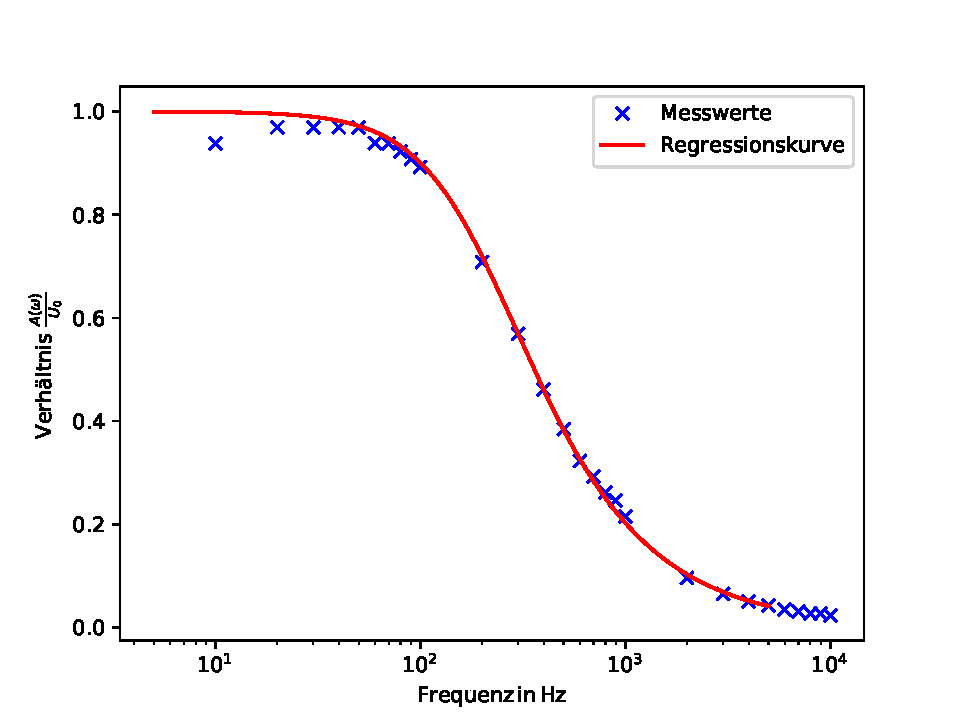
\includegraphics[width = 12 cm]{plotamplitude.pdf}
  \caption{Verhältnis der gemessenen Spannungsamplituden $U\ua{C}$ und der
           Ausgangsspannung $U\ua{0}$ aus Tabelle \ref{tab:MessungB} aufgetragen
          gegen die Frequenz $\omega$}
  \label{fig:Messungb}
\end{figure}
\newpage
\subsection{Bestimmung der Zeikonstante über die Phasenverschiebung}
Die Phasenverschiebung wird mit Formel \ref{eqn:phi} bestimmt. Dafür werden gemessenen Werte der
Nulldurchgänge beider Schwingungen $a$ und die Schwingungsdauer $b$ mithilfe des Oszilloskops
bestimmt.

Für das RC- Glied ergibt sich durch die Phasenverschiebung der Wert von:
\begin{equation*}
  RC = (0.000502 \pm 0.00025) \, \su{s} .
\end{equation*}
\begin{table}
  \centering
  \caption{Messwerte für die Parameter a und b sowie die berechnete Phasenverschiebung}
  \label{tab:Phasenverschiebung}
  \begin{tabular}{c c c c}
    \toprule $\omega \,\, in  \,\, \su{Hz}$ & $a \,\, in \,\, \su{ms}$ &
             $b \,\, in \,\, \su{ms}$ & $\varphi \,\, in \,\, \su{rad}$ \\
    \midrule
     10 & 0.720 & 100.00 & 0.045 \\
     20 & 0.800 & 48.80 & 0103 \\
     30 & 0.800 & 32.40 & 0.155 \\
     40 & 0.792 & 24.40 & 0.204 \\
     50 & 0.784 & 20.00 & 0.246 \\
     60 & 0.776 & 16.60 & 0.294 \\
     70 & 0.768 & 14.20 & 0.340 \\
     80 & 0.760 & 12.40 & 0.385 \\
     90 & 0.744 & 11.00 & 0.424 \\
    100 & 0.736 & 9.80 & 0.472 \\
    200 & 0.624 & 5.04 & 1.005 \\
    300 & 0.516 & 3.28 & 0.998 \\
    400 & 0.440 & 2.52 & 1.097 \\
    500 & 0.376 & 2.00 & 1.181 \\
    600 & 0.328 & 1.72 & 1.198 \\
    700 & 0.292 & 1.48 & 1.240 \\
    800 & 0.262 & 1.24 & 1.328 \\
    900 & 0.238 & 1.08 & 1.385 \\
    1000 & 0.216 & 1.00 & 1.357 \\
    2000 & 0.118 & 0.48 & 1.545 \\
    3000 & 0.080 & 0.33 & 1.523 \\
    4000 & 0.062 & 0.25 & 1.558 \\
    5000 & 0.050 & 0.20 & 1.571 \\
    6000 & 0.042 & 0.17 & 1.552 \\
    7000 & 0.037 & 0.14 & 1.661 \\
    8000 & 0.032 & 0.13 & 1.547 \\
    9000 & 0.029 & 0.11 & 1.656 \\
    10000 & 0.026 & 0.10 & 1.634 \\
    \bottomrule
  \end{tabular}
\end{table}
\begin{figure}
  \centering
  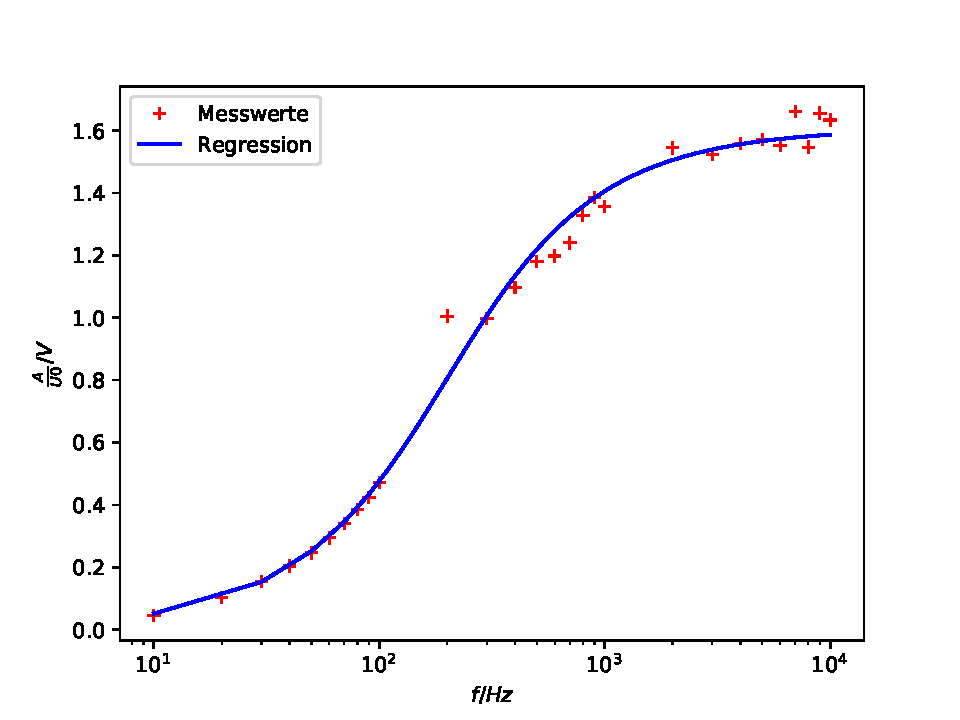
\includegraphics[width = 12 cm]{Plot2.pdf}
  \caption{Phasenverschiebung aufgetragen gegen die Frequenz}
  \label{fig:Messungc}
\end{figure}

\newpage
\subsection{Der RC-Kreis als Integrator}
Im letzten Teil des Experiments soll die Integratoreigentschaften des RC-Kreises anhand
drei verschiedener Spannungen überprüft werden. Dabei stellt die gelbe Spannungskurve die eingespeiste
Generatorspannung und die blaue Spannungskurve die dazugehörige integrierte Kondensatorspannung dar.

Zuerst wird eine Rechteckspannung eingespeist deren Integration eine Dreiecksspannung liefert.
\begin{figure}
  \centering
  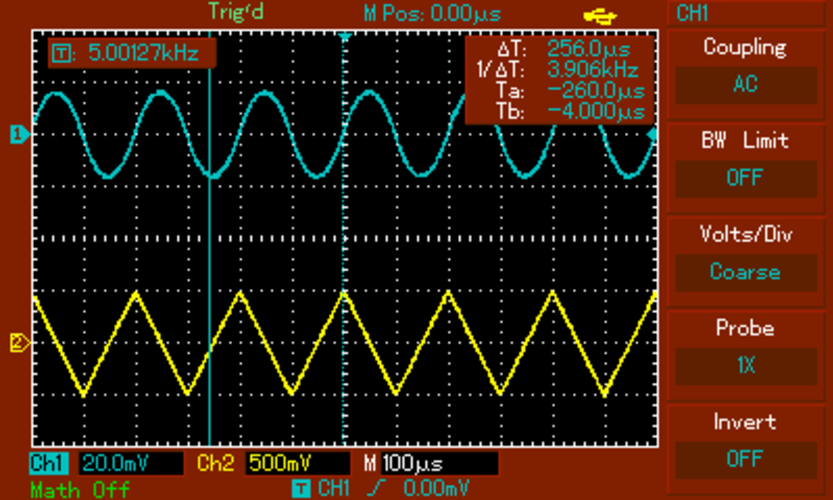
\includegraphics{rechteck.pdf}
  \caption{Anliegende Rechteckspannung bei dem RC-Kreis}
  \label{fig:Rechteck}
\end{figure}

\newpage
Bei einer anliegenden Dreiecksspannung ergibt sich durch die Integration eine Sinusspannung.
\begin{figure}
  \centering
  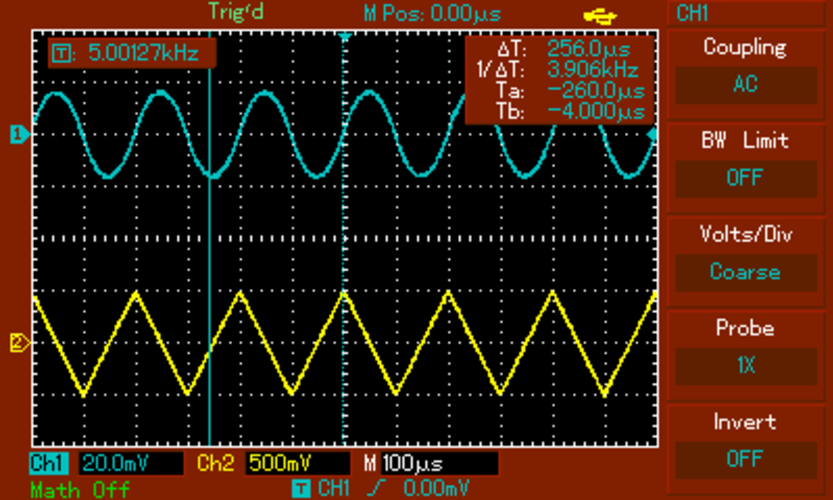
\includegraphics{dreieck.pdf}
  \caption{Anliegende Dreieckspannung bei dem RC-Kreis}
  \label{fig:Dreieck}
\end{figure}

\newpage
Entsprechend der Integration einer Sinusspannung sollte sich durch den RC-Kreis eine Cosinusspannung einstellen,
was beim Thermodruck in Abbildung \ref{fig:Sinus} zu sehen ist.
\begin{figure}
  \centering
  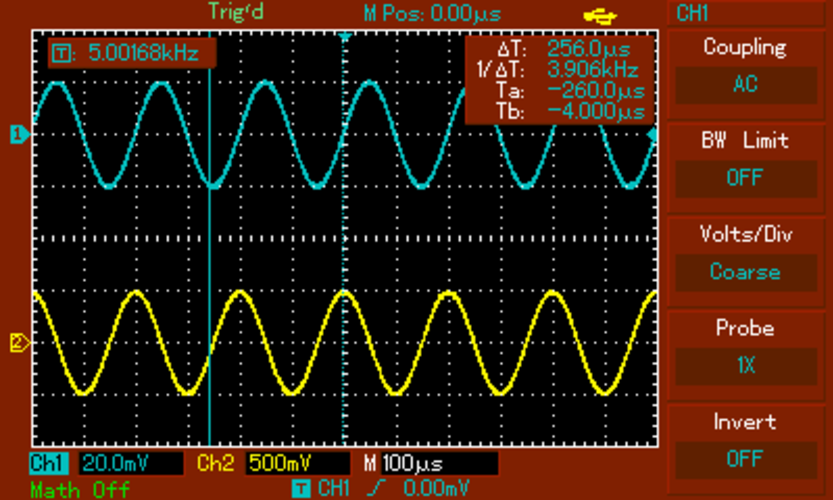
\includegraphics{sinus.pdf}
  \caption{Anliegende Sinusspannung bei dem RC-Kreis}
  \label{fig:Sinus}
\end{figure}
